\chapter{Proteini} % Main chapter title
\label{Chapter2}

Sva živa bića sastoje se iz ćelija. U ćelijama se neprestano odvijaju različiti procesi u kojima učestvuju nukleinske kiseline (dezoksiribonukleinka kiselina - DNK i ribonukleinska kiselina - RNK) i proteini. Unutar molekula DNK šifrovan je genetski materijal koji sadrži uputstva za sintezu proteina. 

Proteini su makromolekuli koji igraju mnoge kritične uloge u organizmu. Sačinjavaju više od 50\% suvog dela ćelije i važni su za njenu izgradnju i funkcionisanje. Kontrakcija mišića, strukturna podrška, ubrzavanje i usporavanje hemijskih reakcija, odbrana od virusa i bakterija samo su neke od mnogobrojnih uloga koje proteini obavljaju \cite{radivojac, doktJK}.


\section{Sinteza proteina}

DNK sadrži informacije koje su neophodne ćeliji za izgradnju veoma važnog tipa molekula - proteina. Proteini se sintetišu prilikom genske ekspresije i to u dva koraka: transkripcija i translacija (slika \ref{fig:synthesis}).  Prvi korak je dekodiranje genske poruke, prilikom čega se od DNK sekvence dobija RNK sekvenca. U sastav obe nukleinske kiseline ulazi 4 nukleotida i oni su prikazane u tabeli \ref{tab: nucleotides}. S obzirom da su tri nukleotidne baze iste, proces transkripcije sastoji se iz zamene svakog molekula T molekulom U. 


\begin{figure}[h]
	\centering
	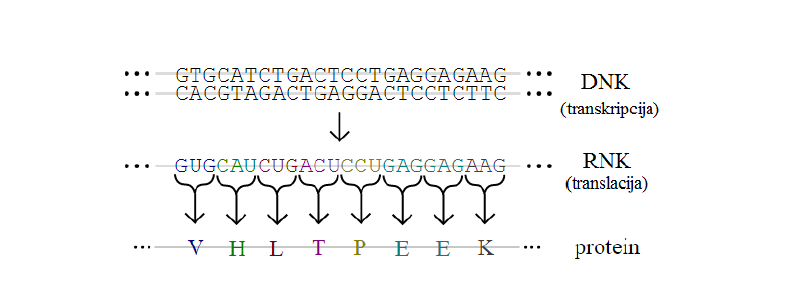
\includegraphics[width=\textwidth]{Figures/protein_synthesis.png}
	\caption{Prikaz procesa sinteze proteina \cite{doktJK}.}
	\label{fig:synthesis}
\end{figure}


\begin{table}[H]
	\centering
	\begin{tabular}{|c|c|c|c|c|}
		\hline
		DNK & adeinin (A) & guanin (G) & citozin (C) & timin (T) \\
		\hline
		RNK & adeinin (A) & guanin (G) & citozin (C) & uracil (U) \\
		\hline             
	\end{tabular}
	\caption{Prikaz nukleinskih kiselina sa nukeotidima koji ih grade}
	\label{tab: nucleotides}
\end{table}


Sledeći korak, proces translacije, jeste grupisanje aminokiselina kako bi se dobio protein. Genetski kod se čita u grupama od 3 nukleotida koje nazivamo \textit{kodoni}. Svaki kodon odgovara tačno jednoj aminokiselini ili služi da označi kraj sekvence (stop kodon). Na primer, kodon \textbf{GUA} kodira aminokiselinu valin, dok kodon \textbf{UAG} označava kraj sekvence. Na slici \ref{fig:codons} je dat šematski prikaz svih kodona i odgovarajućih aminokiselina. Jedan po jedan, kodoni se prevode u odgovarajuće aminokiseline čime se dobija sekvenca aminokiselina koja čini protein \cite{BMBG, synthesisOnl}.

\begin{figure}[h]
	\centering
	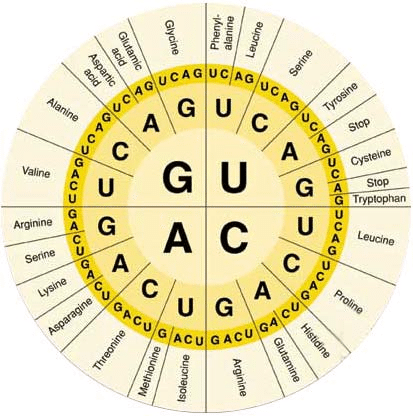
\includegraphics[width=0.6\textwidth]{Figures/codons_chart.png}
	\caption{Prikaz kodona i odgovarajućih aminokiselina}
	\label{fig:codons}
\end{figure}


\section{Aminokiseline}

Aminokiseline su organska jedinjenja koja se sastoje od karboksilne grupe ($COOH$), aminogrupe ($NH_2$) i bočnog lanca (R-grupa) koji je vezan za $\alpha$-ugljenikov atom i karakterističan je za svaku aminokiselinu. Postoji 20 standardnih aminokiselina i one su prikazane u tabeli \ref{tab: aminoacids}. Pod standardnim aminokiselinama podrazumevaju se one aminokiseline za koje postoji najmanje jedan specifičan kodon u genetskom kodu \cite{biochemestry5, biohUdz, straus}.


\begin{table}
	\centering
	\begin{tabular}{|lcc|lcc|}
		\hline
		Aminokiselina & Oznaka & Simbol & Aminokiselina & Oznaka & Simbol \\
		\hline
		Alanin & ALA & A & Arginin & ARG & R  \\
		Asparagin & ASN & N & Asparaginska kiselina & ASP & D \\
		Cistein & CYS & C & Glutamin & GLN & Q  \\
		Glutaminska kiselina & GLU & E & Glicin & GLY & G  \\
		Histidin & HIS & H & Izoleucin & ILE & I  \\
		Leucin & LEU & L & Lisin & LYS & K  \\
		Metionin & MET & M & Fenilalanin & PHE & F  \\
		Prolin & PRO & P & Serin & SER & S  \\
		Treonin & THR & T & Triptofan & TRP & W  \\
		Tirosin & TYR & Y & Valin & VAL & V \\
		\hline             
	\end{tabular}
	\caption{Prikaz standardnih aminokiselina sa oznakama i simbolima}
	\label{tab: aminoacids}
\end{table}

~ \\
\noindent Aminokiseline možemo podeliti u nekoliko grupa prema osobinama bočnog lanca \cite{biochemestry5, biohUdz, bioinf}:

\begin{enumerate}
	\item \textbf{aminokiseline sa nepolarnim bočnim lancem}\\
	Bočni lanac ovih aminokiselina ne može da otpušta niti da vezuje protone, kao ni da učestvuje u vodoničnim ili jonskim vezama. Zbog svoje nepolarnosti, one su hidrofobne i obično popunjavaju praznine u unutrašnjosti proteina čime doprinose oblikovanju njegove strukture. U ovu grupu ubrajamo 7 standardnih aminokiselina: alanin, valin, leucin, izoleucin, metionin, fenilalanin, triptofan. 
	
	\item \textbf{aminokiseline sa nenaelektrisanim polarnim bočnim lancem}\\
	R-grupa aminokiselina iz ove grupe može da gradi vodonične veze sa molekulima vode što ih čini rastvorljivijim u odnosu na aminokiseline iz prethodne grupe. Zbog polarnosti, ove aminokiseline se obično nalaze na spoljašosti proteina. Ova grupa obuhvata 6 standardnih aminokiselina i to: serin, treonin, tirozin, asparagin, glutamin i cistein. 
	
	\item \textbf{aminokiseline sa naelektrisanim polarnim bočnim lancem}\\
	U ovu grupu spadaju veoma hidrofilne aminokiseline zbog čega se one nalaze na površini proteina. Dodatno ih možemo podeliti na kisele i bazne aminokiseline. Kisele imaju jednu karboksilnu grupu više i imaju negativno naelektrisanje, dok su bazne aminokiseline pozitivno naelektrisane. Asapraginska i glutaminska kiselina su kisele aminokiseline, a lizin, histidini i arginin spadaju u bazne aminokiseline.  
	
	\item \textbf{konformaciono važne aminkiseline}\\
	Preostale dve standardne aminokiseline, glicin i prolin se po svojoj strukuturi razlikuju od ostalih. Glicin nema bočni lanac i može da se prilagođava konformacijama koje su nedostupne drugim aminokiselinama. Prolin sadrži jedan heterociklički prsten i u svojoj strukuturi sadrži sekundarnu amino grupu. 
\end{enumerate}



Bilo koje dve aminokiseline mogu izgraditi veći molekul, dipeptid, formiranjem peptidne veze između njih. Peptidna veza se ostvaruje između atoma ugljenika iz karboksilne grupe i atoma azota iz amino grupe. Peptidne veze omogućavaju stvaranje lanaca aminokiselina, tzv. polipeptida. Peptidna veza nastaje reakcijom dve aminokiseline pri čemu se spajaju karboksilna grupa jedne sa amino grupom druge aminokiseline uz izdvajanje vode. Prilikom tog vezivanja pojavljuje se niz koji se zove kičma polipeptidnog lanca koji čine ugljenikov atom karboksilne grupe, atom azota aminogrupe i $\alpha$-ugljenikov atom. To je osnovni niz i isti je za sve proteine, a oni se međusobno razlikuju po bočnim lancima aminokiselina \cite{biohUdz, bioinf}.


Peptide možemo podeliti prema broju aminokiselina koje sadrže i to na oligopeptide i polipeptide. Oligopeptidi su sačinjeni od najviše 10 aminokiselina, dok polipeptidi sadrže do 100 aminokiselina. Jedinjenja sa više od 100 aminokiselina u lancu spadaju u proteine \cite{biohUdz}.



\section{Struktura proteina}

U sastav proteina ulazi 20 standardnih aminokiselina. Sekvenca aminokiselina, koja se formira peptidnim vezama, specifična je za svaki protein. Ona je primarni izvor informacija o proteinu i njegovoj funkciji. Složenost proteinske strukture najbolje se analizira kroz četiri nivoa: primarna, sekundarna, tercijerna i kvaterna struktura \cite{biochemestry5}.

\paragraph{Primarna strktura} Jedinstveni redosled aminokiselina koje su povezane peptidnom vezom kako bi formirale protein čini primarnu strukturu proteina. Proteini koji imaju slične sekvence često imaju i slične osobine i funkcije. Zbog toga je poređenje sekvenci prvi korak u izučavanju proteina. Razumevanje primarne sekvence je bitno zbog mnogih genetskih bolesti koje za posledicu imaju proteine sa neispravnim sekvencama što vodi do pogrešnog savijanja i nefunkcionalnog proteina \cite{biochemestry5, biohUdz, bioinf}.

\paragraph{Sekundarna struktura} Polipeptidni lanac ne zauzima bilo kakav oblik u prostoru već ima opšti raspored aminokiselina koje se u lancu nalaze jedna blizu druge. Taj raspored označava sekundarnu strukturu proteina i podrazumeva savijanje ili uvijanje polipeptidnog lanca. Lanac može da uzme oblik $\alpha$-heliksa (engl. $\alpha$-helix), $\beta$-traka (engl. $\beta$-sheet) ili $\beta$-okreta (engl. $\beta$-turn). $\alpha$-heliks je periodična struktura u kojoj se kičma proteina spiralno uvrće, a bočni lanci aminokiselina izviruju izvan nje. $\beta$-traka formiraju se kao parovi lanaca aminokiselina koji se uzdužno vezuju vodoničnim vezama. $\beta$-okret menja pravac polipeptidnog lanca čime mu pomaže dobije kompaktan, loptast oblik \cite{biochemestry5, bioinf, PSF}.

\paragraph{Tercijarna struktura} 
Prostorna struktura čitavog molekula proteina predstavlja ternarnu strukturu. Hidrofobni bočni lanci nepolarnih aminokiselina teže da budu unutar molekula proteina zaštićeni od vode, dok se kisele i bazne aminokiseline obično nalaze na površini proteina pošto su hidrofilne. $\alpha$-heliksi i $\beta$-listovi služe da obezbede maksimalan broj vodoničnih veza u unutrašnjosti molekula, čime sprečavaju da se molekuli vode vežu za hidrofilne grupe i time naruše integritet proteina \cite{biochemestry5, biohUdz}.


\paragraph{Kvaternarna struktura} Mnogi proteini su formirani grupisanjem više savijenih polipeptidnih lanaca. Pojedinačnu komponentu nazivamo podjedinica. One mogu biti međusobno različite ili potpuno iste. Raspored ovih podjednica predstavlja kvaternarnu strukturu.  U kvaternarnu strukturi podjedinice se međusobno drže zajedno nekovalentnim interakcijama i kovalentnim vezama  \cite{doktJK, biochemestry5, PSF}.


\section{Uloga proteina}


Proteini su najbrojniji i funkcionalno najrazličitiji molekuli u živom svetu. Svaki od njh ima veoma važnu ulogu u organizmu. Na primer:

\begin{itemize}
	\item Enzimi su proteini koji olakšavaju hemijske reakcije. Učestvuju u skoro svim reakcijama u ćelijama i pomažu u izgradnji novih molekula.
	
	\item Antitela su proteini koje proizvodi imuni sistem da bi pomogli u odstranjivanju stranih supstanci i kako bi se borile protiv infekcija. Oni se vezuju za nepoznate čestice, poput bakterija i virusa čime brane telo 
	
	\item Kontrakcijski proteini učestvuju u kontrakcijama mišića i kretanju.
	
	\item Strukturni proteini su vlaknasti i obezbeđuju strukturu i podršku ćelijama. Učestvuju u izdgradnji kose, noktiju, kože, kostiju, itd.
	
	\item Transportni proteini prenose molekule kroz telo.
	
	\item Hormonski proteini prenose signale kako bi upravljali biološkim procesima među ćelijama, tkivima i organima.
	
	\item Skladišni proteini čuvaju aminokiseline za kasniju upotrebu \cite{fspOnl, roleOnl, nlmOnl}.
	
\end{itemize}
 
 

